\section{Make-a-Video}
\label{sec:make_a_video}

Make-a-Video \cite{make_a_video} (2022) by Meta AI is a text-to-video model. Similar to Video-LDM, Make-a-Video extends the text-to-image (T2I) knowledge to diffusion-based text-to-video (T2V) model through spatiotemporally factorized diffusion model. In addition, it \textbf{doesn't require pairs of text-video data}, which allows unsupervised video training, which in turn allows to scale to larger quantities of video data.

They present super-resolution strategies in space and time to generate higher spatial-resolution and higher frame rate video clips, provided a text prompt. They \textbf{leverage image priors} due to the complexity of modeling videos, which simplifies the learning process.

One of the downsides of Make-a-Videos, is that because its trained on unlabeled video data, it can't learn associations between text and phenomenons that can only be inferred in videos (for example: moving hands from left to right). They left this to future work.

The model has 3 main stages:

\begin{itemize}
    \item \textbf{Training a T2I model on text-image pairs}. This model is variation of DALL-E 2 \cite{dalle_2} (section \ref{sec:dalle_2}) by OpenAI.
    \item Converting the T2I model to T2V model by \textbf{adding 3D convolutions and temporal attention layers in the U-Net}, so the model can understand video data. It becomes a T2V model.
    \item \textbf{Unsupervised training of the T2V model on video data} (no text-to-video data is needed), which is very attractive.
\end{itemize}



\subsection{Architecture \& Method}

\begin{figure}
    \centering
    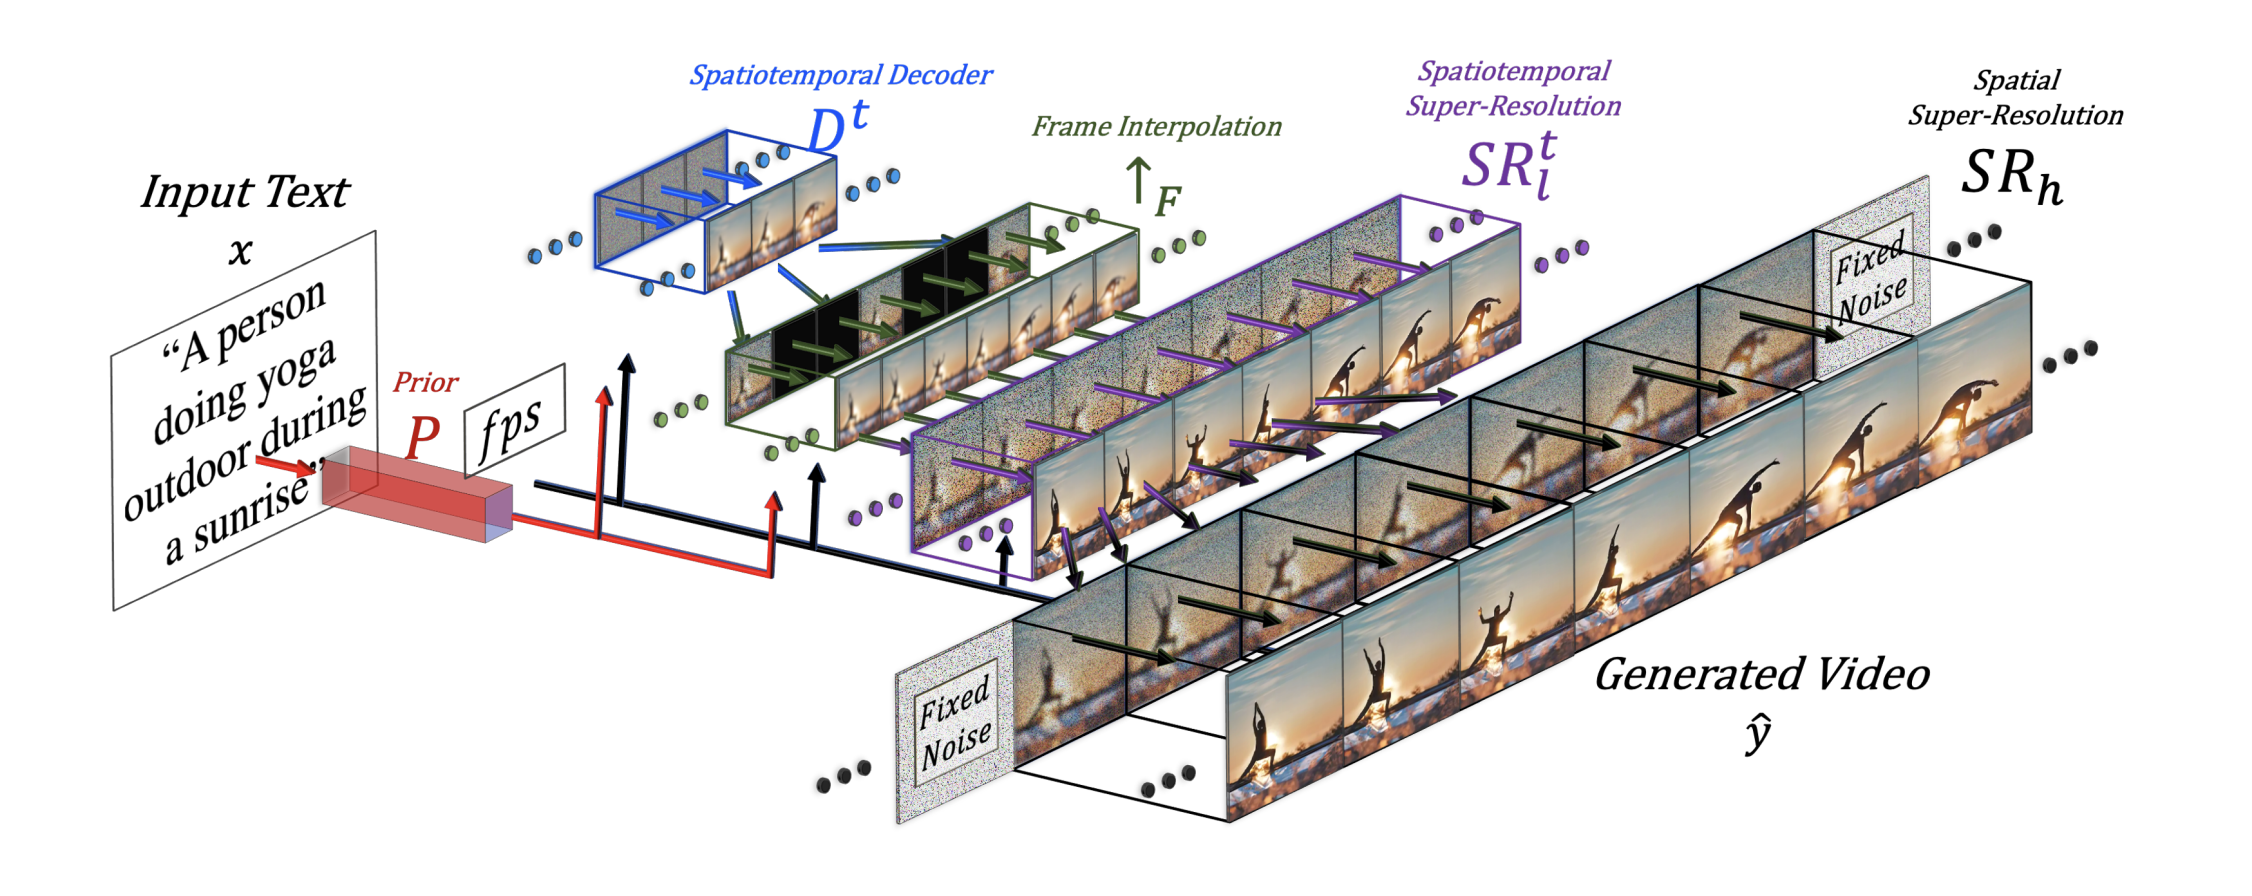
\includegraphics[width=1\textwidth]{images/make_a_video/overview.png}
    \caption{Make-a-Video model high-level architecture overview (after adding temporal layers). The T2I model doesn't have "fps" input, the decoder generates only a single image, there is no interpolation network, and has two spatial-super-resolution networks, and no spatio-temporal super-resolution network, since in image we don't deal with the temporal axis \cite{make_a_video}.}
    \label{fig:make_a_video_overview}
\end{figure}

In figure \ref{fig:make_a_video_overview}:

\begin{itemize}
    \item The model input is text prompt $x$ and "fps" (frames per second).
    \item $\hat{x}$ is the BPE encoded text.
    \item The \textbf{CLIP text encoder} $C_x$ (not shown in the figure) is used to translate the text prompt $x$ into text embeddings $x_e$, which are fed to the prior network $\textcolor{Maroon}{P}$.
    \item The \textbf{image embedding prior} $\textcolor{Maroon}{P}$ translates these text embeddings $x_e$ into image embeddings $y_e$.
    \item The \textbf{spatio-temporal decoder $\textcolor{blue}{D^t}$} generates 16 $64\times 64$ frames, conditioned on these image embeddings $y_e$.
    \item These 16 images are interpolated into higher fps by the \textbf{frame interpolation model $\textcolor{OliveGreen}{\uparrow_F}$}, through masked interpolation prediction, as we saw in previous papers.
    \item Then these frames are increased in spatial resolution to $256\times 256$ by the \textbf{spatiotemporal super-resolution model $\textcolor{Plum}{SR_l^t}$}.
    \item And finally increased to resolution $768\times 768$ by \textbf{spatial super-resolution model $SR_h$}. The final output is high-spatiotemporal-resolution video $\hat{y}$.
\end{itemize}

The formal mathematical formulation of the Make-a-Video inference is as follows:

\begin{equation}
    \hat{y_t} = \text{SR}_h \circ \textcolor{Plum}{\text{SR}_l^t} \circ \textcolor{OliveGreen}{\uparrow_F} \circ \textcolor{blue}{D^t} \circ \textcolor{Maroon}{P} \circ \left( \hat{x}, C_x (x) \right)
    \label{eq:make_a_video_inference}
\end{equation}

where $\hat{x}$ is the BPE encoded text tokens.







\subsection{The T2I model}

The T2I model is based on the core components of the OpenAI paper \cite{dalle_2}. In this paper, OpenAI created a model that is called unCLIP (commonly known as DALL-E 2). See section \ref{sec:dalle_2} for more details. They first trained the T2I model, and only then they apply factorization on the T2I model to create the T2V model. We will discuss this T2I model here and in the next section, and explain how they transfer this spatial knowledge to video in section \ref{sec:make_a_video_expanding_t2i_to_video}.

The researchers note that after the inference (equation \ref{eq:make_a_video_inference}), they then downsample the image to $512\times 512$ using bicubic interpolation for cleaner aesthetics.







\subsubsection{DALL-E 2}
\label{sec:dalle_2}

DALL-E 2 by OpenAI \cite{dalle_2} is a diffusion-based T2I model, which leverages contrastive models like CLIP for image generation. They proposed a two-stage model: 

\begin{itemize}
    \item a prior network $P(z_i | y)$ that generates CLIP image embeddings $z_i$ conditioned on captions
    \item and a diffusion based decoder $P(x | z_i, y)$ that generates images $x$ conditioned on these image embeddings $z_i$, and optionally the captions $y$.
\end{itemize}

\begin{figure}
    \centering
    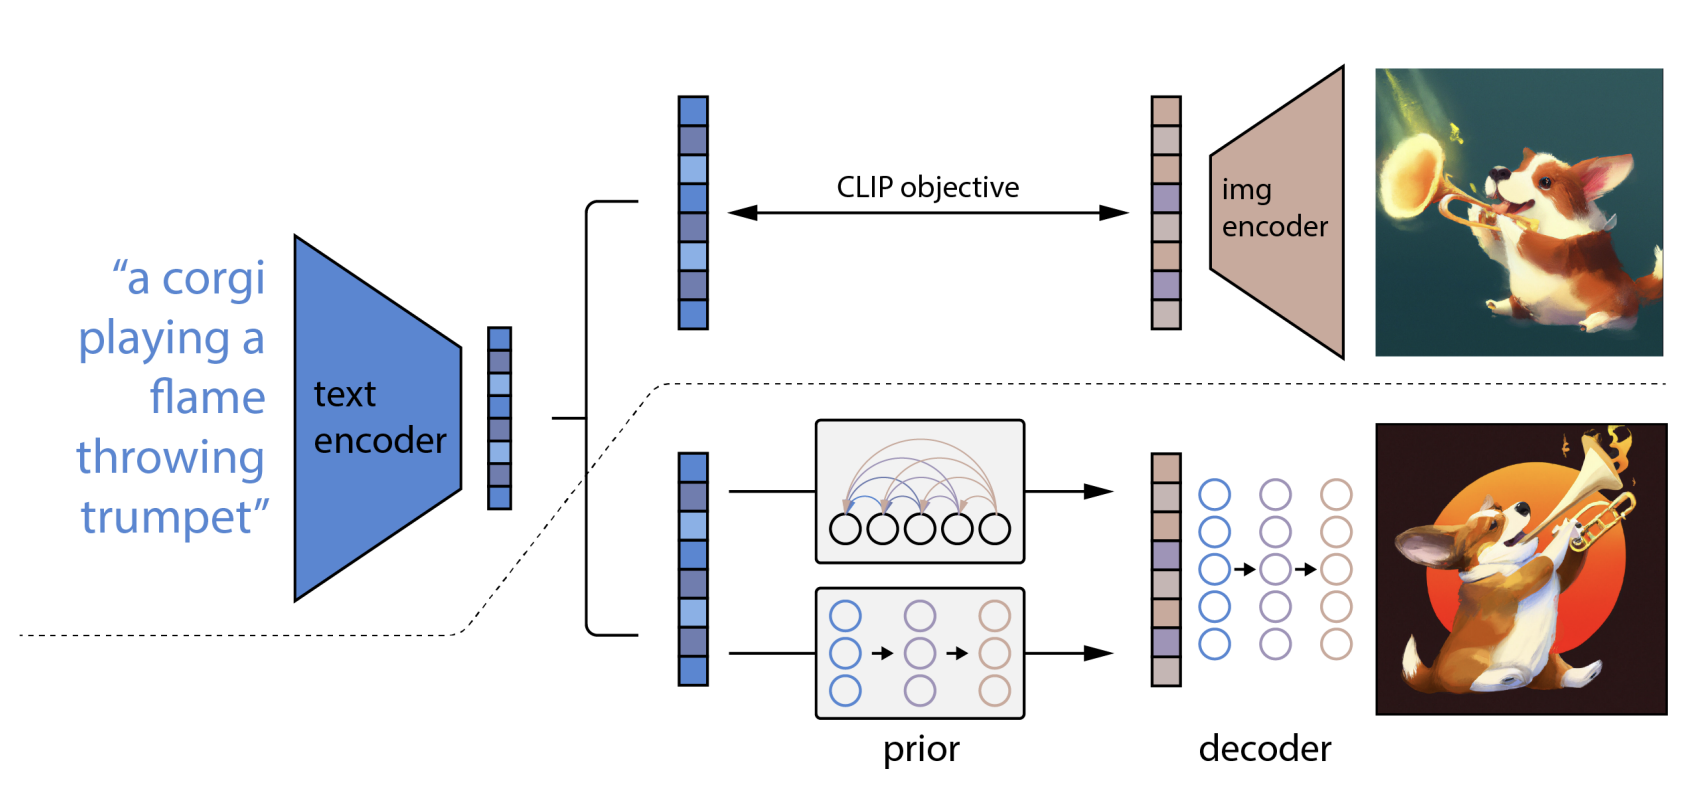
\includegraphics[width=0.7\textwidth]{images/make_a_video/dalle_2.png}
    \caption{High level overview of unCLIP (DALL-E 2) \cite{dalle_2} by OpenAI. The top figure shows the training objective of DALL-E 2, and the bottom figure shows the inference process. The prior model takes the CLIP text embeddings $z_t$ and generates image embeddings $z_i$. Then the decoder takes in image embeddings $z_i$ and generates the final image \cite{make_a_video}.}
    \label{fig:make_a_video_dalle2_overview}
\end{figure}

In figure \ref{fig:make_a_video_overview}, we can see the training objective of DALL-E 2 and the inference process. The decoder acts as inverted CLIP encoder. Given inputs $(x, y)$ where $x$ are images and $y$ are their caption, then $z_i$ is the corresponding CLIP image embeddings and $z_t$ is the CLIP text embeddings.

\begin{itemize}
    \item \textbf{Input}: the training dataset is pairs $(x,y)$ of images $x$ and captions $y$.
    
    \item \textbf{Output}: a generated image $x$ given a caption $y$.

    \item \textbf{CLIP encoder} is applied to the text $x$ and caption $y$ to get text and image embeddings $z_i$ and $z_t$ respectively.
    
    \item \textbf{Training objective}: the text embedding $z_t$ (the blue vector in figure \ref{fig:make_a_video_overview}) should match the CLIP image embeddings $z_i$ (the brown vector in figure \ref{fig:make_a_video_overview}).
    
    \item \textbf{The prior network} maps the text embeddings $z_t$ to a \textit{distribution} of possible image embedding vectors $z_i$. In their experiments, they tried two different prior networks:
        \begin{itemize}
            \item \textbf{Autoregressive} prior: the image embedding $z_i$ is converted to a sequence of discrete codes and predicted autoregressively conditioned on the caption $y$. This network is based on the transformer architecture.
            \item \textbf{Diffusion} based prior where the latent vector $z_i$ is modeled using Gaussian diffusion model conditioned on caption $y$. The diffusion model is a decoder-only transformer, instead of a standard U-Net, similar to Diffusion Transformer \cite{diffusion_transformer}.
        \end{itemize}
    
    \item \textbf{Decoder network}: given image embeddings $z_i$, the unCLIP network generates the final image; the decoder is considered inverse of CLIP encoder, or just "unCLIP" (hence the name). They also used classifier-free guidance to improve the quality of the generated images.
    
    \item \textbf{Sampling in DALL-E}: to sample an image we need to first sample $z_i$ using the prior network, and then sample $x$ using the decoder (given $z_i$).
    
    \item \textbf{Super-resolution}: they also trained two SR diffusion-based networks to upsample the final generated image from $64\times 64$ to $256\times 256$ and finally to $1024\times 1024$.
\end{itemize}

\textbf{x-prediction}: In the prior network, instead of predicting the noise directly ($\epsilon$-prediction), they chose to predict the unnoised $z_i$ directly (called $x$-prediction).





\subsection{Expanding the T2I model to video domain}
\label{sec:make_a_video_expanding_t2i_to_video}

The researchers modify the T2I model and transfer the image knowledge to video domain by expanding the 2D conditional network into the temporal dimension.

In short, they support the temporal dimension by adding 3D convolutions temporal attention layers in the U-Net backbone of the T2I diffusion model. The \textbf{fully-connected layers doesn't need factorization since they are agnostic to structured spatial and temporal information}.



\subsubsection{Spatiotemporal layers}

The spatiotemporal decoder $\textcolor{blue}{D^t}$ now \textbf{generates 16 RGB frames} of $64\times 64$ resolution, instead of one frame.

They added a new network: \textbf{frame interpolation network} $\textcolor{OliveGreen}{\uparrow_F}$ which increases the fps by interpolating on the 16 frames from the spatiotemporal decoder (as seen in figure \ref{fig:make_a_video_overview}).

\textbf{Hallucination}: the super-resolution model involves hallucinating information. In order not to have flickering artifacts, the hallucination must be consistent across frames. As a result, $\text{SR}_l^t$ operates across spatial and temporal dimensions.

They also modified the spatial layers of the super-resolution network $\text{SR}_l$ to spatiotemporal super-resolution network $\textcolor{red}{\mathbf{\text{SR}_l^t}}$. \textbf{But chose not to operate in the temporal dimension} in $\text{SR}_h$. The reason being because of memory and compute constraints higher in the pipeline.

In order to consistent detail hallucination across frames, in $\text{SR}_h$ they use the same noise initialization for each frame.



\subsubsection{Pseudo-3D convolutional layers}

Because 3D convolutional layers are very compute and memory expensive, the researchers opt to go with pseudo 3D convolutional layers.

In \cite{chollet2017xception}, the authors proposed a method to replace 3D convolutions with pseudo-3D convolutions. In this method they decouple the processing of spatial and temporal dimensions, which they call "depthwise separable convolution layers". In Make-a-Video they say that in addition to the more compute efficient convolutions they also want to retain the previously learned spatial knowledge of the T2I model.

\textbf{First they apply the 2D convolution on spatial axis and only then they apply 1D convolution on the temporal axis}. This facilitates information sharing between the spatial and temporal axes.

The pseudo-3D convolutional layer is defined as:

\[ 
\text{Conv}_{\text{P3D}} (h) := \text{Conv}_{\text{1D}} (
    \text{Conv}_{\text{2D}} (h) \circ T
) \circ T \]

where $h \in \mathbb{R}^{B\times C\times F\times H\times W}$ is an input tensor, where $B,\ C,\ F,\ H,\ W$ are the batch, channels, frames, height and width respectively, and $\circ T$ is the transpose operator which swaps between spatial and temporal dimensions.

\begin{figure}
    \centering
    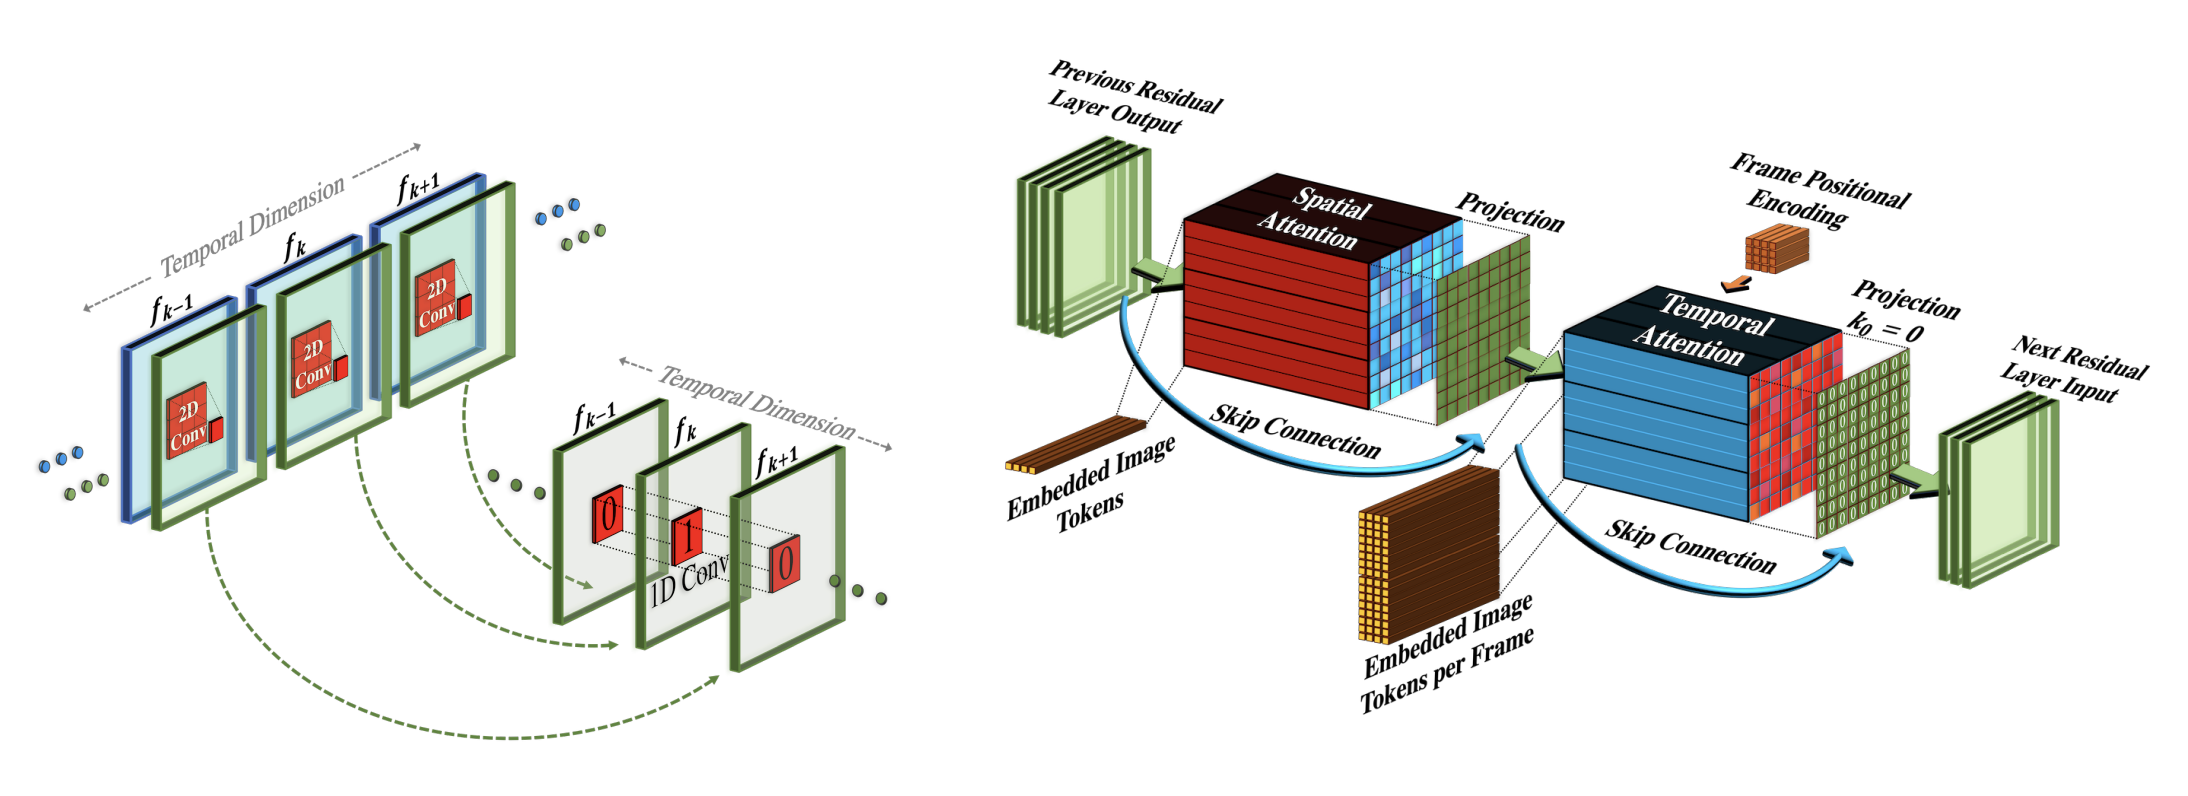
\includegraphics[width=0.7\textwidth]{images/make_a_video/pseudo_3d.png}
    \caption{Initialization and architecture of pseudo-3D convolutional and attention layers. Left: Pseudo-3D convolution and initialization. Right: Pseudo-3D attention and initialization \cite{make_a_video}.}
    \label{fig:make_a_video_pseudo_3d_conv_and_attention}
\end{figure}

\textbf{Spatiotemporal initialization}: In figure \ref{fig:make_a_video_pseudo_3d_conv_and_attention} we can see the pseudo-3D convolutional layer initialization. After applying 2D spatial convolutions they apply 1D temporal convolution. \textbf{The temporal 1D convolution layer is initialized as the identity function, it performs no transformation on the input data initially}. This way the network relies on the already learned spatial features. \textbf{The temporal consistency will be learned at a later stage}, where the model is trained on video dataset.






\subsubsection{Pseudo-3D attention layers}

Adding the temporal dimension to the attention layers is computationally infeasible. They follow the work of \cite{video_diffusion_models} (Video U-Net), similar to how \textbf{Imagen-Video} works (in Imagen-Video paper they also mentioned that they use the work of Video U-Net).

After each pre-trained spatial attention layer they stack a pseudo-3D temporal attention layer. 

Given tensor a tensor $h$ the \texttt{flatten} operation flattens the spatial dimension to: 

\[ 
h' \in \mathbb{R}^{B\times C\times F\times \mathbf{\textcolor{red}{HW}}} 
\] 

and \texttt{unflatten} operation is the inverse operation. The pseudo-3D attention layer is defined as:

\[ \text{ATTN}_{\text{P3D}} (h) = \text{unflatten} 
(\text{ATTN}_{\text{1D}} 
(\text{ATTN}_{\text{2D}} 
(\text{flatten} (h)) \circ T) \circ T) 
\]

\textbf{Spatiotemporal initialization}: To allow for smooth spatiotemporal initialization, $\text{ATTN}_{\text{2D}}$ is initialized from the pre-trained T2I model and the $\text{ATTN}_{\text{1D}}$ is initialized as the identity function (see figure \ref{fig:make_a_video_pseudo_3d_conv_and_attention}).

\textbf{FPS conditioning}: similar to \cite{cogvideo}, they added additional conditioning parameter $\text{fps}$, which enables additional augmentation method that deals with limited volume of training videos and provides more control over the generated video at inference time.





\subsection{Frame interpolation network}

The frame interpolation network $\textcolor{OliveGreen}{\uparrow_F}$ increases number of frames by interpolation or pre/post extrapolation. In addition to RGB channels, they add the binary mask channel (0 or 1) indicating which frames masked during training on masked interpolation. The model is conditioned on $\text{fps}$ which enable multiple temporal upsample rates at inference. For extrapolation, they can use the same strategy.




\subsection{Training}

The prior network is trained on text-image pairs, and isn't fine-tuned on videos.

The decoder, prior and two SR networks are first trained on images alone, and then temporal layers are added and then they fine-tune them over unlabeled video data.





\subsection{Experiments}

\subsubsection{Datasets}

To train the T2I model, they used 2.3B subset of Laion-5b \cite{laion_5b} of image-text pairs.

To train the T2V model, they used:
\begin{itemize}
    \item WebVid-10M \cite{webvid_10m} text-to-video dataset
    \item and a 10M subset from HD-VILA-100M \cite{hd_vila_100m}
\end{itemize}

The decoder, interpolation network and $\text{SR}_h$ were trained on WebVid-10M.

In addition $\text{SR}_h$ is trained on HD-VILA-10M.

\textbf{Evaluation}: They conducted evaluation on UCF-101 \cite{ucf_101} and MSR-VTT \cite{msr_vtt} in zero-shot setting. The researchers also used \textbf{DrawBench prompts from Imagen for human evaluation}.



\subsubsection{Quantitative Results}

\begin{figure}[h]
    \centering
    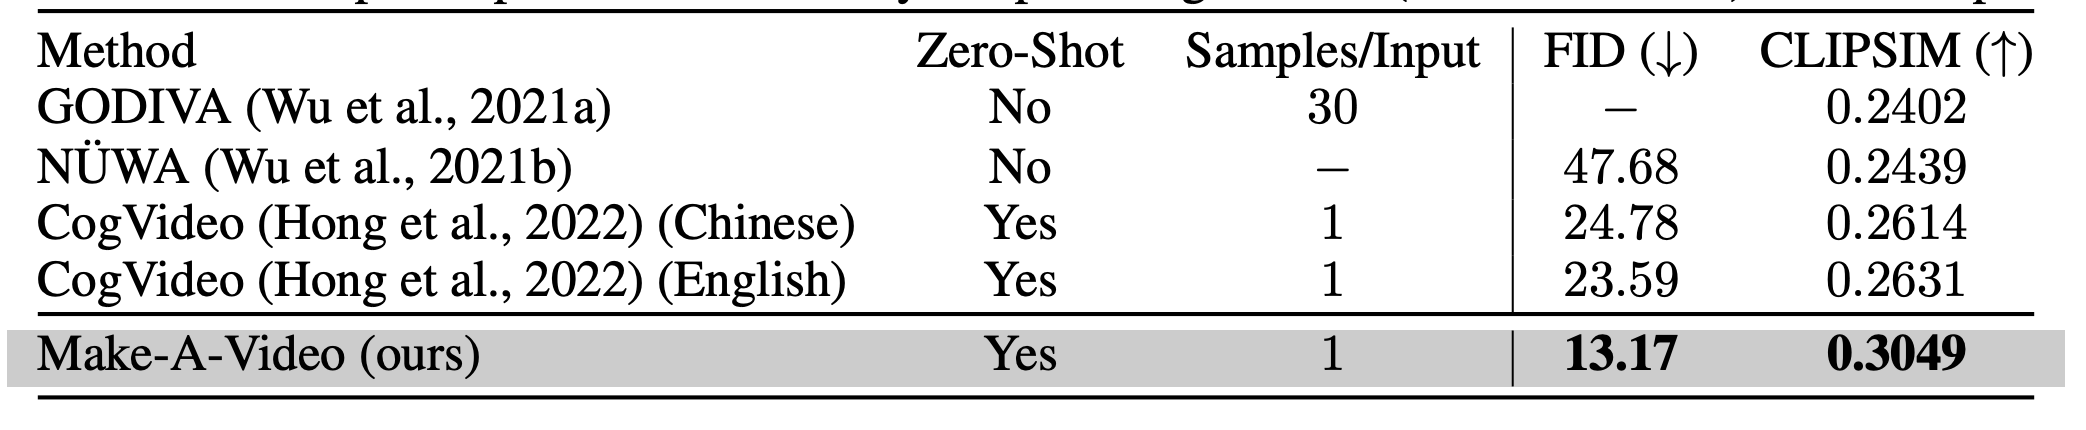
\includegraphics[width=0.7\textwidth]{images/make_a_video/zero_shot_eval.png}
    \caption{Make-a-Video significantly outperforms all state-of-the-art T2V generation models in zero-shot setting on MSR-VTT \cite{msr_vtt} dataset of video  and captions in both FID and CLIP-SIM score \cite{make_a_video}.}
    \label{fig:make_a_video_zeroshot_eval}
\end{figure}

Evaluation on MSR-VTT is shown in figure \ref{fig:make_a_video_zeroshot_eval}.

\begin{figure}[h]
    \centering
    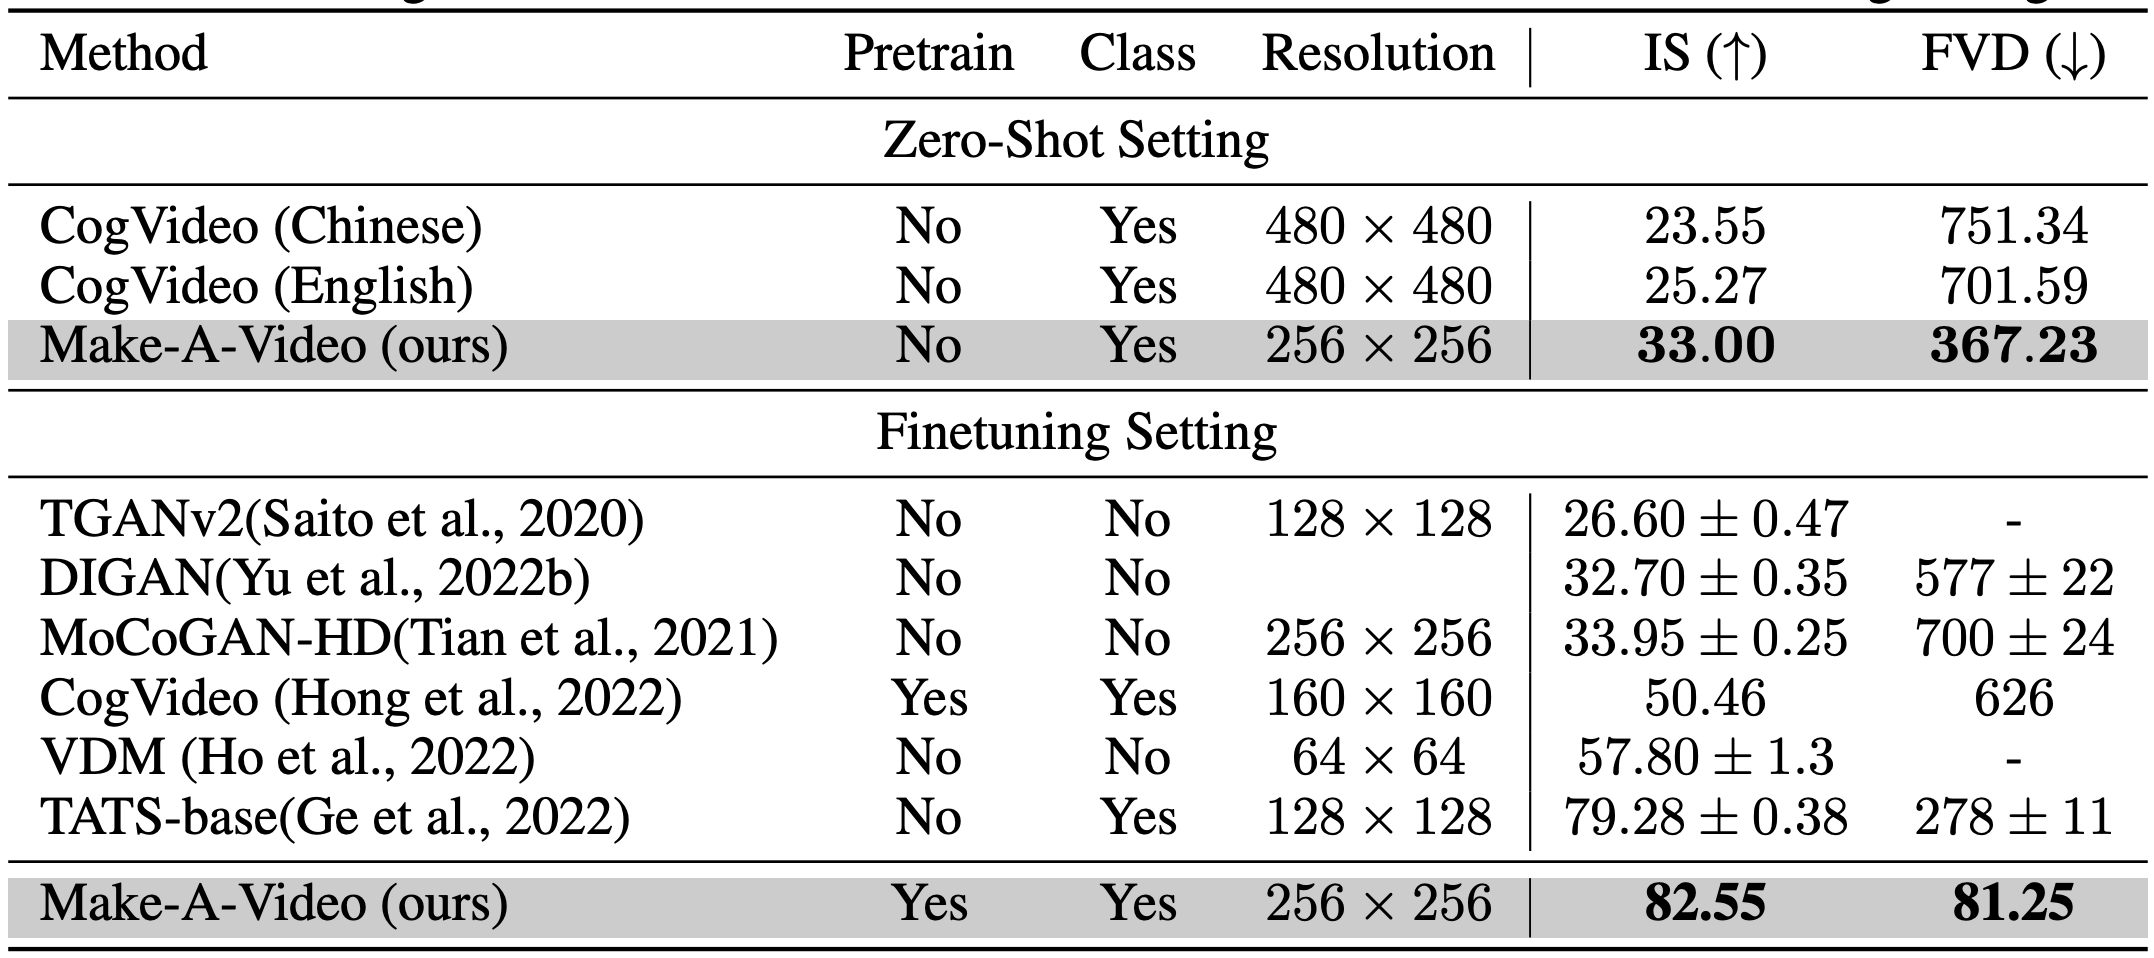
\includegraphics[width=0.7\textwidth]{images/make_a_video/ucf_101.png}
    \caption{Zero-shot and fine-tuning evaluation on UCF-101 dataset \cite{make_a_video}.}
    \label{fig:make_a_video_ucf_101}
\end{figure}

Evaluation on UCF-101 is shown in figure \ref{fig:make_a_video_ucf_101}..

\begin{figure}[h]
    \centering
    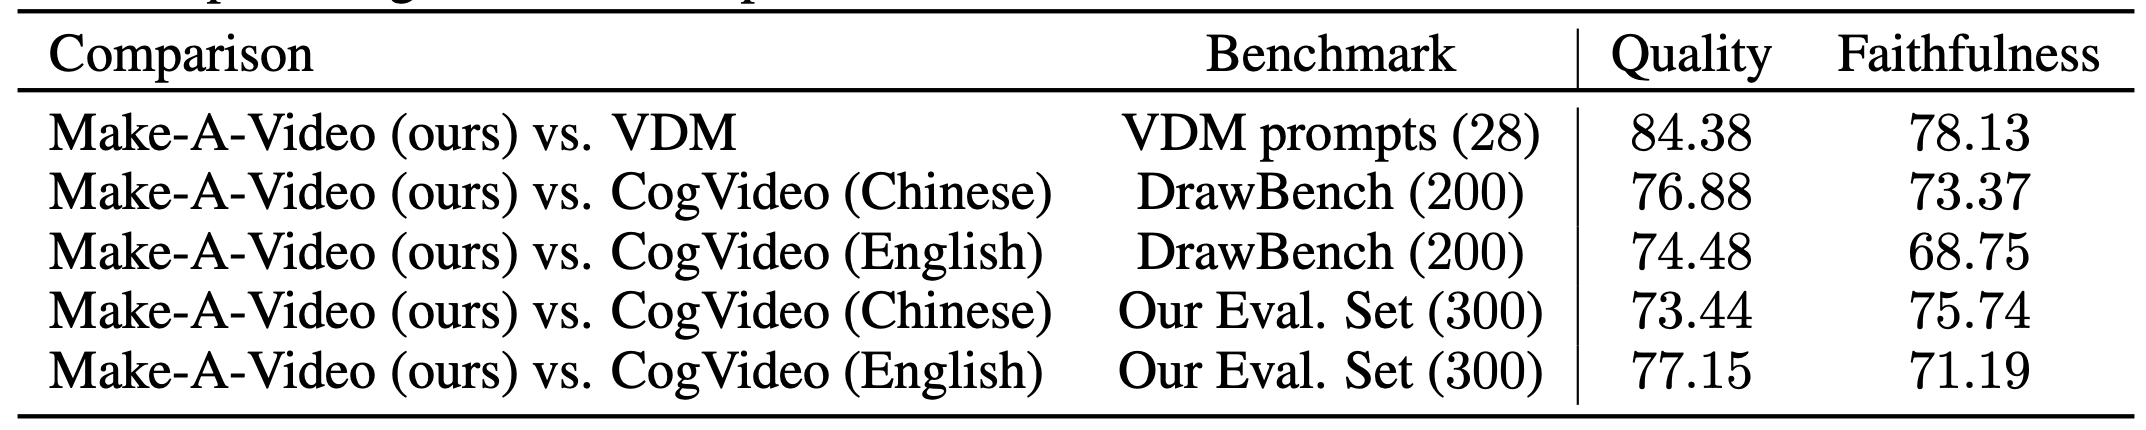
\includegraphics[width=0.7\textwidth]{images/make_a_video/eval.png}
    \caption{Human evaluation on DrawBench. The number indicates amount of videos compared in each evaluation \cite{make_a_video}.}
    \label{fig:make_a_video_human_eval}
\end{figure}

Human evaluation is shown in figure \ref{fig:make_a_video_human_eval}. They ask humans which video (out of two videos chosen randomly) is higher quality. For faithfulness, they show the text description of the video in addition to the video, and ask which video has better correspondence with the text. CogVideo is the only public zero-shot T2V model.



\subsubsection{Qualitative Results}

\begin{figure}
    \centering
    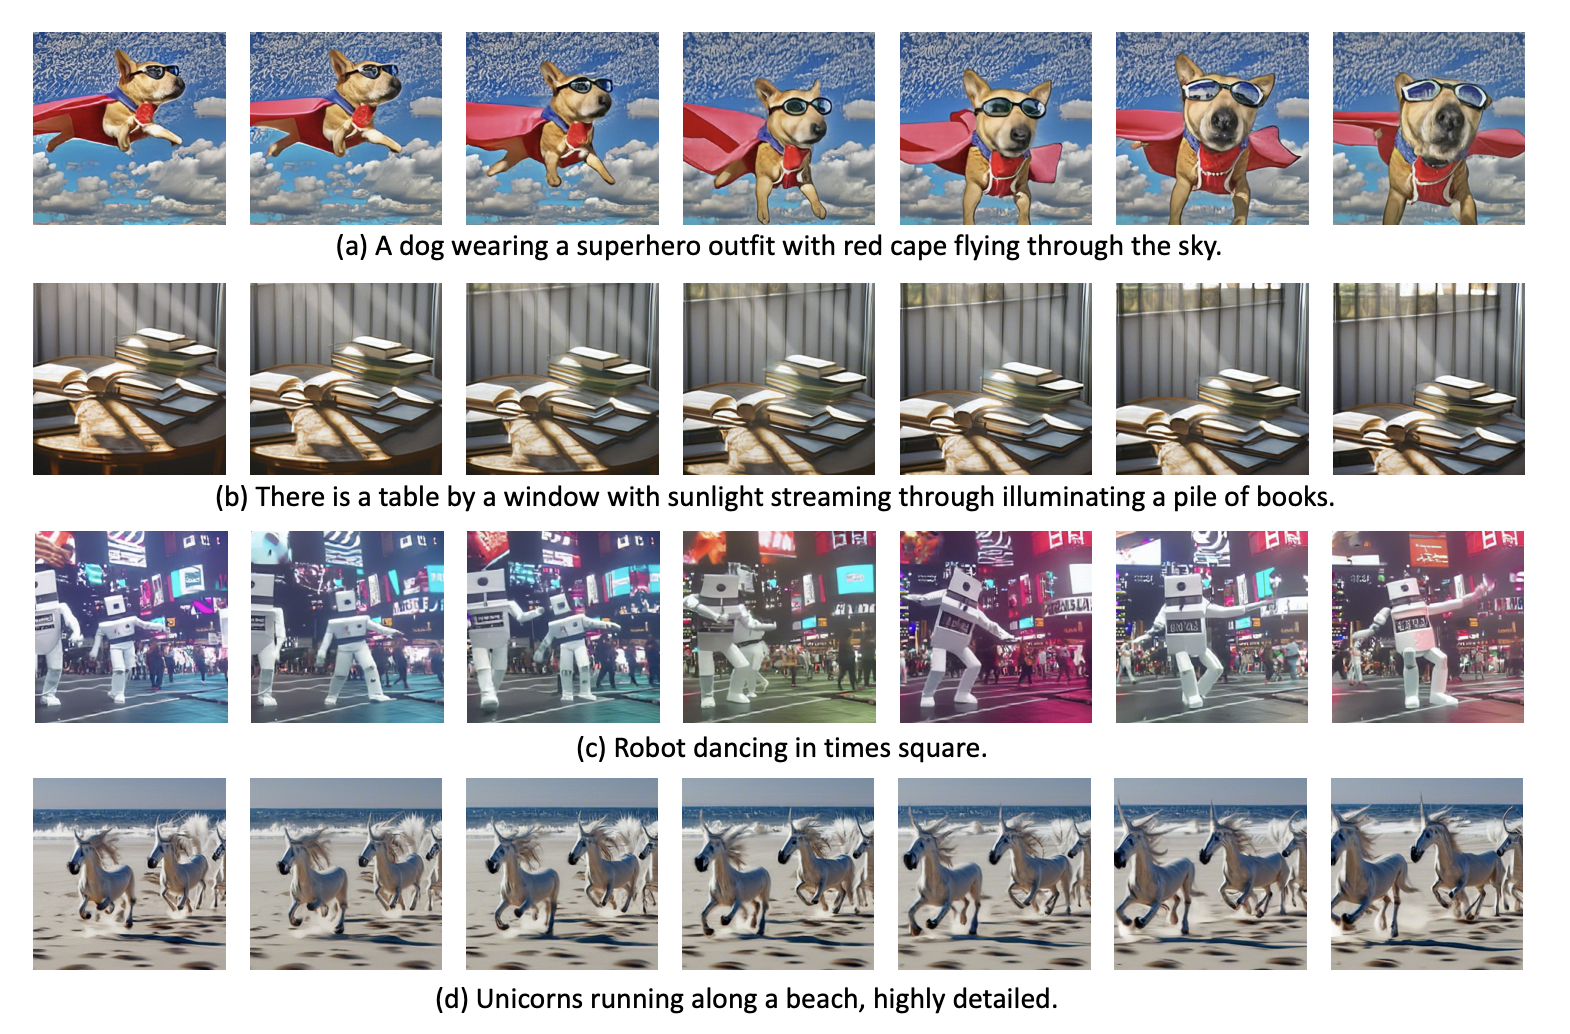
\includegraphics[width=0.7\textwidth]{images/make_a_video/examples.png}
    \caption{Examples of T2V samples of Make-a-Video \cite{make_a_video}.}
    \label{fig:make_a_video_examples}
\end{figure}

\begin{figure}
    \centering
    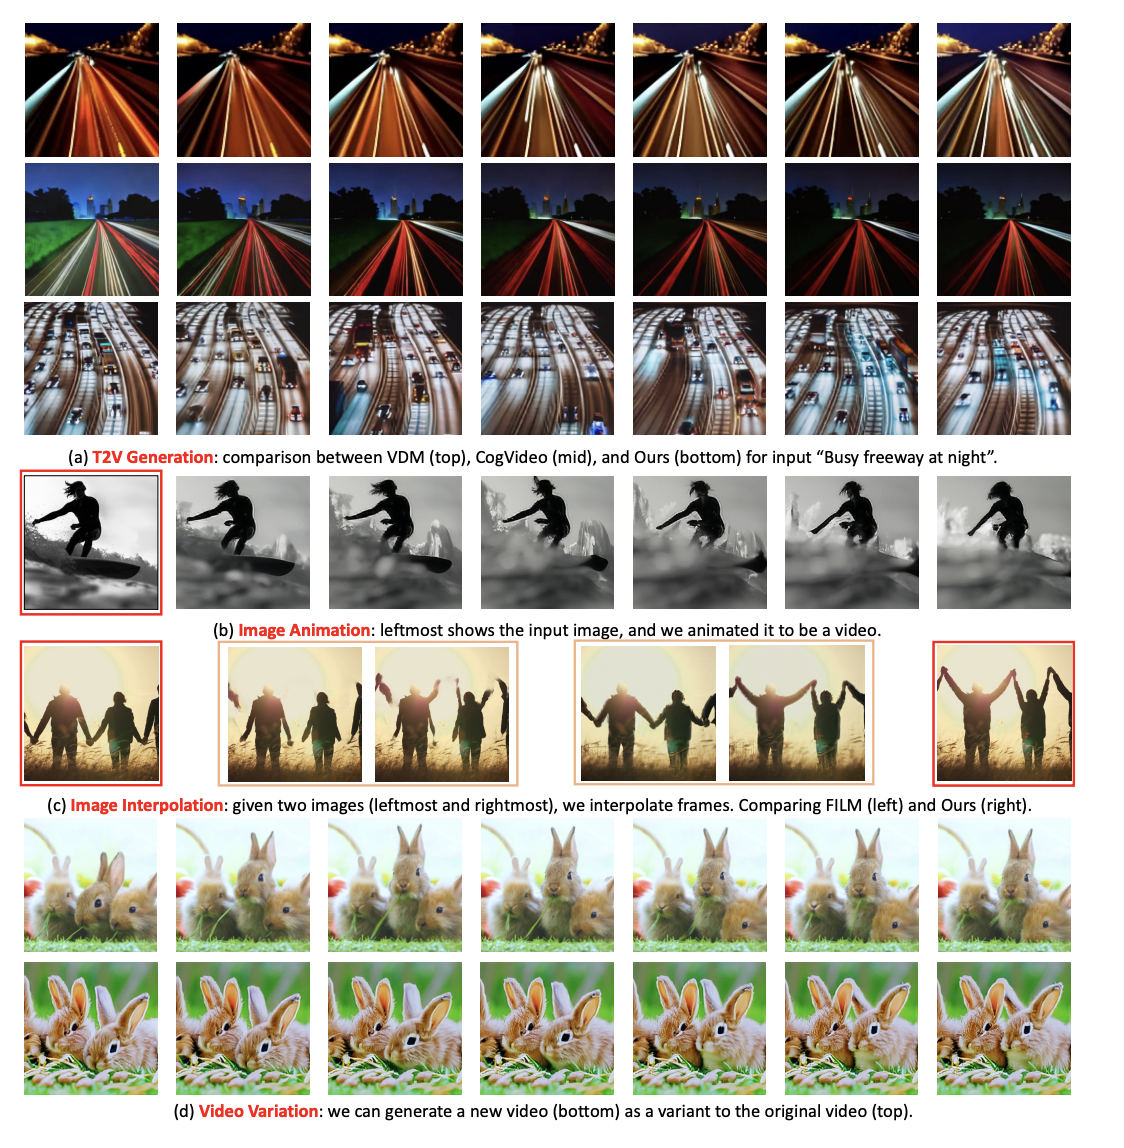
\includegraphics[width=0.7\textwidth]{images/make_a_video/examples2.png}
    \caption{Various qualitative results comparisons and applications. FILM by Google Research is a frame-interpolation model \cite{film}  \cite{make_a_video}.}
    \label{fig:make_a_video_examples2}
\end{figure}

In figure \ref{fig:make_a_video_examples2} (c) we see the interpolation network works better than FILM \cite{film}.

